\documentclass[conference]{IEEEtran}

\usepackage[T1]{fontenc}
\usepackage[utf8]{inputenc}
\usepackage{amsmath,amssymb,bm}
\usepackage{booktabs,multirow,array,tabularx,ragged2e}
\usepackage{graphicx}
\usepackage{xcolor}
\usepackage{cite}
\usepackage{microtype}
\usepackage{siunitx}
\usepackage{enumitem}
\usepackage[hidelinks]{hyperref}

\newcolumntype{C}[1]{>{\centering\arraybackslash}p{#1}}
\newcolumntype{L}[1]{>{\RaggedRight\arraybackslash}p{#1}}
\renewcommand{\arraystretch}{1.18}
\setlength{\tabcolsep}{4pt}

\title{YogaLLaVA: Geometry-Conditioned Vision--Language Reasoning for Yoga Pose Understanding}

\author{
\IEEEauthorblockN{Manav Barot, Sadamori Kojaku}
\IEEEauthorblockA{
School of Systems Science and Industrial Engineering\\
State University of New York (SUNY), Binghamton, NY, USA
}
}

\begin{document}
\maketitle

\begin{abstract}
A body posture is arbitrarily linked to its cultural or social meaning.
Vision--language models fall short in inferring meaning from appearance when subtle physical differences carry substantially different meanings.
This failure can endorse harmful form in physical therapy or exercise and misrepresent postures whose meaning matters to the communities that practice them.
We address this limitation by pairing images with explicit, measured body geometry and conditioning a vision--language model on that geometry to capture meaning changes hidden in small visual differences.
Using yoga as a challenging domain, we introduce \textbf{YogaAlign}, a benchmark that extends Yoga-82 with measured body geometry paired with question--answer annotations.
Building on YogaAlign, we train \textbf{YogaLLaVA V3}, a vision--language model that conditions on body geometry through new learnable tokens encoding the measurements of the geometric structure.
Instead of guessing or rounding, YogaLLaVA V3 expresses precise numeric measurements in generated language by leaving a placeholder token at each numeric position and replacing it with a continuous value from an additional regression head.
YogaLLaVA V3 produces the correct number of numeric measurements in 86.1\% of evaluation samples, a 26\% relative gain over the best image-only baseline, Qwen2.5-VL-7B (68.1\%).
On the shared common-success subset, it achieves a mean absolute error of $17.65^\circ$, a 59\% reduction relative to the best baseline, LLaVA-1.5-7B ($42.80^\circ$).
More broadly, our results show that making body geometry explicit, instead of leaving it implicit, helps models learn the arbitrary link between appearance and its cultural or social meaning.
\end{abstract}

\begin{IEEEkeywords}
vision--language models; yoga pose understanding; 3D human mesh recovery; geometry grounding; instruction tuning; Yoga-82
\end{IEEEkeywords}
\section{Introduction}
\label{sec:intro}

The cultural or social meaning of a body posture is arbitrarily linked to its physical appearance.
Postures that look nearly identical can carry substantially different meanings.
A model that reads appearance alone cannot determine which meaning applies.
Recovering the meaning requires the measured configuration of the body.

When a vision--language model misses the subtle physical differences that separate such postures, it can endorse harmful form in physical therapy or exercise by confirming a misaligned joint as correct.
The same failure can misrepresent postures whose meaning matters to the communities practicing them.

Inferring meaning from appearance therefore requires explicit, measured body geometry expressed in language.
Human pose analysis is commonly formulated as keypoint localization~\cite{cao2019openpose,sun2019deep}, skeleton recovery, or action recognition.
These tasks provide perceptual representations but do not answer natural-language questions about configuration, such as which side is more flexed or how a geometric property should be described in words.
Such questions require a model to connect image evidence with explicit body measurements and linguistic reasoning.

Yoga is a particularly demanding setting for this problem.
Many asanas are distinguished by small differences in joint flexion, limb elevation, trunk orientation, and bilateral symmetry.
Yoga-82~\cite{verma2020yoga82} provides a large and visually diverse benchmark for fine-grained recognition across 82 pose categories.
Its supervision is limited to hierarchical category labels.
It does not provide reconstructed 3D bodies, interpretable geometric descriptors, or question--answer annotations that connect a specific image to its measured configuration.

Recent progress in monocular human mesh recovery and visual instruction tuning offers a path toward such supervision.
SAM 3D Body recovers articulated body structure under the Momentum Human Rig representation from a single image~\cite{yang2026sam3dbody}.
Models such as LLaVA learn to follow language instructions conditioned on visual input~\cite{liu2023visual}.
A direct combination, however, leaves two unresolved issues.
First, dense mesh outputs must be converted into compact and interpretable measurements.
Second, continuous geometric values must be integrated into language generation without reducing numeric prediction to unconstrained text-token generation.

We introduce \textbf{YogaAlign}, a benchmark that pairs Yoga-82 images with measured body geometry and question--answer annotations grounded in that geometry.
The geometry comes from SAM 3D Body reconstructions, summarized into a taxonomy of angular, symmetry, trunk, and support descriptors.
The annotations form two sets.
We produce pose-level domain-knowledge QA by evidence-conditioned synthesis from textual sources.
We generate geometry-grounded QA directly from the measurements of each image.

Building on YogaAlign, we train \textbf{YogaLLaVA V3}, a vision--language model that conditions on this geometry during generation.
Ordered \texttt{<GEO>} tokens carry the angular subset of the measurements.
The \texttt{<ANGLE>} mechanism separates the decision to place a numeric slot from continuous scalar regression and feeds the predicted value back into the autoregressive context.
In free-running evaluation, YogaLLaVA V3 produces the correct number of numeric measurements more often than the best baseline (86.1\% of samples versus 68.1\% for Qwen2.5-VL-7B) and achieves lower angular error on the shared common-success subset (a mean absolute error of $17.65^\circ$ versus $42.80^\circ$ for LLaVA-1.5-7B).

We make three contributions.
\begin{itemize}[leftmargin=1.2em,itemsep=2pt,topsep=3pt]
    \item We introduce \textbf{YogaAlign}, a geometry-grounded extension of Yoga-82 containing 3D-derived descriptors and 10,090 instruction-style question--answer pairs across 82 asanas.
    \item We develop a two-part annotation procedure that combines evidence-conditioned yoga-domain knowledge with image-specific geometric measurements, exact angular targets, rule-based validation, and traceable provenance.
    \item We build \textbf{YogaLLaVA V3} on YogaAlign, integrating metric-aware geometry tokens, continuous angle-slot regression over descriptors supplied through those tokens, and scalar feedback into a vision--language decoder, and evaluate both teacher-forced angle regression and free-running generation.
\end{itemize}
Our experiments cover the geometry-grounded set alone.
The domain-knowledge set is released as a training and evaluation resource, and we report no model performance on it.
\section{Related Work}
\label{sec:related}

\noindent\textbf{Pose estimation and body reconstruction.}
Methods that recover body configuration from a single image treat the geometry as their final product.
Two-dimensional estimators localize joint keypoints accurately.
Successive designs fuse multi-scale features~\cite{newell2016stacked,xiao2018simple}, associate keypoints across multiple people~\cite{cao2019openpose}, and adopt high-resolution or transformer backbones~\cite{sun2019deep,xu2022vitpose}.
Parametric body models~\cite{loper2015smpl} extend this recovery to three-dimensional pose and shape, and regressors estimate both from one image~\cite{kanazawa2018end,kolotouros2019spin,li2022cliff,goel2023humans}.
SAM 3D Body extends this line to reconstruction of the full body~\cite{yang2026sam3dbody}.
We instead treat reconstruction as annotation, converting its dense outputs into interpretable measurements that ground our language supervision.

\noindent\textbf{Action quality and pose correction.}
Action quality assessment judges how well a movement is performed without stating how the body is configured.
These methods score performance across varied actions~\cite{lei2019survey,parmar2019action} and rehabilitation exercises~\cite{liao2020deep}, and yoga systems go further to report the joint angles behind a pose prediction~\cite{dittakavi2022posetutor}.
Those angles explain a verdict on correctness.
Our supervision expresses the configuration in language, with every numeric statement traceable to an explicit, image-specific measurement.

\noindent\textbf{Vision--language models and VQA.}
Vision--language models link appearance to the words that describe it.
Contrastive pretraining over image--text pairs establishes this link at scale~\cite{radford2021clip}.
Later systems couple frozen image encoders with language models~\cite{alayrac2022flamingo,li2023blip2} and tune the pair to follow visual instructions~\cite{liu2023visual,dai2023instructblip,wang2024qwen2vl}.
The benchmarks behind this progress ask about objects, attributes, and relations whose answers are visible in the image~\cite{goyal2017vqav2,hudson2019gqa}.
A body posture, by contrast, is arbitrarily linked to its cultural or social meaning.
Postures that look nearly identical can carry substantially different meanings, and appearance statistics alone cannot determine which meaning applies.
Recovering the meaning therefore requires the measured configuration of the body.

\noindent\textbf{Human pose datasets.}
To our knowledge, no existing pose dataset pairs an image with measured body geometry and language grounded in that geometry.
Large collections annotate two-dimensional keypoints at scale~\cite{lin2014coco,andriluka2014mpii}.
Motion capture supplies three-dimensional pose under controlled conditions~\cite{ionescu2014human36m}, and later work extends it to in-the-wild video~\cite{vonMarcard2018}.
Closest to our setting, Yoga-82 offers a visually diverse benchmark of 82 asanas~\cite{verma2020yoga82}.
Its supervision stops at hierarchical category labels.
YogaAlign builds on that diversity and supplies the missing pairing of reconstruction-derived measurements and language grounded in them.
\section{YogaAlign Dataset}
\label{sec:dataset}

We construct \textbf{YogaAlign}, a geometry-grounded vision--language benchmark that extends Yoga-82 with reconstructed 3D body structure, geometric measurements, and instruction-style question--answer (QA) annotations.
The benchmark supports reasoning beyond pose recognition, including joint-angle interpretation, bilateral comparison, regional alignment analysis, and pose-specific instructional knowledge.
At a high level, we construct it in three stages as follows.
We reconstruct a 3D body from each image, then extract geometric descriptors, and finally generate two QA sets grounded in either pose-level textual knowledge or image-specific geometry.

\subsection{Source Images and 3D Body Reconstruction}
\label{subsec:source_reconstruction}

\noindent\textbf{Yoga-82 source dataset.}
YogaAlign is built on Yoga-82~\cite{verma2020yoga82}, which contains 28,478 images spanning 82 fine-grained yoga-pose categories.
The images were collected from online sources and exhibit substantial variation in viewpoint, background, illumination, clothing, practitioner appearance, and execution style.
Yoga-82 is therefore a challenging setting for geometry-aware reasoning.
Many poses differ through small changes in limb articulation, trunk orientation, balance, or bilateral symmetry.
The original dataset, however, provides only RGB images and category labels.
It does not include 3D body structure, geometric measurements, or language annotations.

\noindent\textbf{Monocular body reconstruction.}
We recover a 3D body representation from each Yoga-82 image using the pretrained SAM 3D Body model~\cite{yang2026sam3dbody}.
Given an image $I$, the model predicts an articulated body and surface mesh under the Momentum Human Rig (MHR) representation.
We retain the predicted mesh vertices and anatomical keypoints required by the subsequent measurement stage.
Fig.~\ref{fig:sam3d_examples} shows representative reconstructions.

\begin{figure*}[!t]
    \centering
    \includegraphics[width=0.98\textwidth]{_ALL_CLASSES_GRID.png}
    \caption{Representative SAM 3D Body reconstructions for images from
    Yoga-82. The examples illustrate the diversity of articulated body
    configurations from which YogaAlign's geometric annotations are derived.}
    \label{fig:sam3d_examples}
\end{figure*}


We treat the recovered bodies as reconstruction-derived geometric proxies.
The reconstructions are not motion capture or manually verified biomechanical ground truth.
Their accuracy may be affected by self-occlusion, foreshortening, loose clothing, unusual inversions, left--right ambiguity, and monocular depth uncertainty.

\subsection{Geometric Measurement Extraction}
\label{subsec:geometric_measurements}

Dense meshes are expressive but too high-dimensional for language-grounded pose analysis.
We therefore reduce each reconstruction to a compact set of anatomically interpretable descriptors (Table~\ref{tab:geometric_metrics}).
We map the raw coordinates to a canonical frame before measurement.
Centering the vertices and keypoints at the mesh centroid removes global translation, and a fixed 3D coordinate convention supplies a consistent vertical axis.

\begin{table*}[t]
\centering
\caption{Taxonomy of geometric descriptors extracted from reconstructed 3D bodies.}
\label{tab:geometric_metrics}
\small
\setlength{\tabcolsep}{4pt}
\renewcommand{\arraystretch}{1.16}
\begin{tabularx}{\textwidth}{L{0.17\textwidth} L{0.25\textwidth} L{0.27\textwidth} X}
\toprule
\textbf{Group} & \textbf{Descriptors} & \textbf{3D computation} & \textbf{Reasoning target} \\
\midrule
Limb flexion &
Left/right knee and elbow flexion &
Interior angles of hip--knee--ankle and shoulder--elbow--wrist triplets &
Degree of flexion and left--right comparison. \\
Limb opening/elevation &
Left/right hip opening and shoulder elevation &
Angles between limb segments and torso-level reference axes &
Hip opening and arm elevation. \\
Trunk geometry &
Trunk tilt, lateral bend, twist, and neck alignment &
Pelvis--shoulder, shoulder--hip, and neck--torso directions &
Uprightness, lateral inclination, axial rotation, and head--torso consistency. \\
Bilateral symmetry &
Knee, elbow, and hip symmetry; shoulder and hip height offsets &
Left--right angular differences and normalized vertical offsets &
Symmetric or asymmetric execution across corresponding body regions. \\
Balance/support &
Stance width and body-center offset &
Ankle separation and horizontal displacement of the mesh center from the pelvis midpoint &
Base of support and lateral body shift. \\
\bottomrule
\end{tabularx}
\end{table*}

\noindent\textbf{Joint-angle descriptors.}
For three anatomical keypoints $\mathbf{p}_a$, $\mathbf{p}_b$, and $\mathbf{p}_c$, we compute the angle centered at $\mathbf{p}_b$ as
\begin{equation}
\theta(a,b,c)=
\cos^{-1}\!\left(
\frac{(\mathbf{p}_a-\mathbf{p}_b)^{\top}(\mathbf{p}_c-\mathbf{p}_b)}
{\lVert\mathbf{p}_a-\mathbf{p}_b\rVert_2
 \lVert\mathbf{p}_c-\mathbf{p}_b\rVert_2}
\right).
\label{eq:joint_angle}
\end{equation}
Knee flexion is measured from the hip--knee--ankle triplet, whereas elbow flexion is measured from the shoulder--elbow--wrist triplet.
Hip opening and shoulder elevation are computed relative to torso-level reference axes.
\begin{figure*}[t]
    \centering
    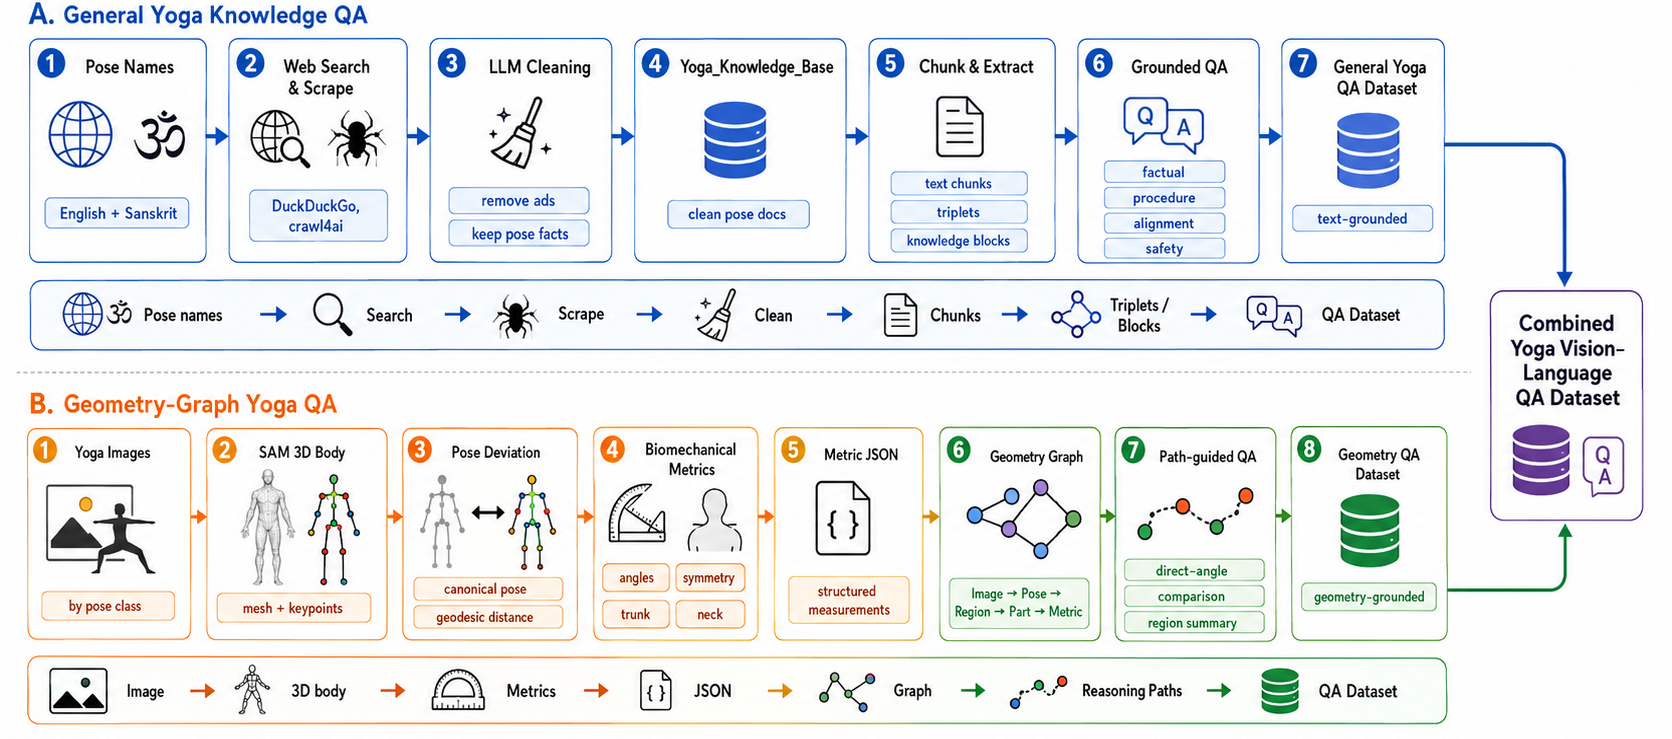
\includegraphics[width=\textwidth]{fig_dataset.png}
    \caption{\textbf{YogaAlign dataset construction.}
    Pose-level domain knowledge and image-specific 3D geometry are processed
    separately to produce the domain-knowledge and geometry-grounded QA
    annotations.}
    \label{fig:dataset_construction}
\end{figure*}
\noindent\textbf{Trunk, symmetry, and support descriptors.}
Trunk measurements are derived from the pelvis--shoulder axis and the shoulder--hip and neck--head directions.
Bilateral descriptors quantify differences between corresponding left and right measurements.
Scale-dependent quantities (stance width, shoulder-height offset, and hip-height offset) are normalized by the vertical extent of the reconstructed mesh to reduce sensitivity to body and reconstruction scale.

\noindent\textbf{Structured metric records.}
Each image is paired with a record containing the descriptor name, anatomical region, numeric value, unit, definition, and discretized interpretation state.
Fixed thresholds map continuous measurements to language-compatible states such as \emph{nearly straight}, \emph{deeply bent}, \emph{upright}, \emph{rotated}, or \emph{asymmetric}.
The states keep the wording consistent, and the underlying numeric values preserve exact supervision.
We use the measurements only as reconstruction-derived alignment indicators for dataset construction.
The measurements are not intended as clinical, diagnostic, or rehabilitation measurements.

\subsection{Question--Answer Annotation}
\label{subsec:qa_generation}

YogaAlign contains two complementary QA sets.
The \emph{domain-knowledge} set captures pose-level semantic and instructional information that cannot be inferred reliably from body geometry alone.
The \emph{geometry-grounded} set expresses image-specific angular evidence extracted from the reconstructed body.
Table~\ref{tab:qa_annotation_overview} in Appendix~\ref{app:annotation_sets} contrasts their evidence sources and supervision targets.


\subsubsection{Domain-Knowledge QA Generation}
\label{subsubsec:domain_qa_generation}

For each of the 82 categories, we collect pose-relevant text from online sources into one document per asana.
We do not generate QA pairs directly from that text.
An extractor $E_{\phi}$ first converts each document chunk $c_i$ into relational facts $R_i$ and structured knowledge units $B_i$, and a generator $G_{\psi}$ conditions on both:
\begin{equation}
\mathcal{Q}^{\mathrm{dom}}_i=G_{\psi}\bigl(c_i,E_{\phi}(c_i,p),p\bigr),
\label{eq:domain_qa}
\end{equation}
where $p$ denotes the pose.
Each accepted item stores its supporting facts, knowledge units, and an evidence phrase, so every answer remains traceable to the source text.
We instruct the extractor to keep only statements supported by the current chunk and to drop claims that a pose cures or treats a medical condition.
Both restrictions are carried by the prompt alone.
No independent check enforces them, and we have not audited the retained records for unsupported medical claims.
Appendix~\ref{app:domain_generation} describes the collection, chunking, and deduplication procedure, and Table~\ref{tab:domain_qa_config} lists the values used.
We fixed these values before generation and did not search over them.

\subsubsection{Geometry-Grounded QA Generation}
\label{subsubsec:geometry_qa_generation}

The second set is generated directly from the measurements associated with an individual image.
We restrict this set to degree-valued descriptors, which provide continuous targets.
Non-angular normalized quantities, including stance width, body-center offset, and shoulder- and hip-height differences, remain part of the geometric annotation taxonomy but are not used for geometry-QA generation or angle-regression supervision.

\noindent\textbf{Metric facts and geometry graphs.}
For image $I$, each valid measurement $m\in\mathcal{M}_I$ is converted to a single metric fact
\begin{equation}
f_m=(r_m,b_m,n_m,v_m,s_m),
\label{eq:metric_fact}
\end{equation}
where $r_m$, $b_m$, and $n_m$ identify the body region, body part, and descriptor.
The entries $v_m$ and $s_m$ store the angular value and its discretized interpretation state.
We organize these facts into a graph $\mathcal{G}_I=(\mathcal{V}_I,\mathcal{E}_I)$ containing image, pose, region, body-part, metric, and interpretation nodes.
Edges encode relations such as image--pose, region--body-part, body-part--metric, and metric--interpretation.
The graph makes the available evidence explicit and supports controlled sampling of different reasoning structures.

\noindent\textbf{Evidence-path construction.}
We derive five path families from each graph (Table~\ref{tab:geometry_path_types}).
A path specifies the selected measurements, the intended reasoning behavior, and the evidence that must appear in the answer.
Direct paths target one descriptor.
Comparison paths pair corresponding left and right descriptors.
Regional paths combine multiple measurements.
Misconception paths verify a proposed condition.
Instructor-observation paths express a notable measured property.

\begin{table*}[t]
\centering
\caption{Evidence-path families for geometry-grounded QA generation.}
\label{tab:geometry_path_types}
\small
\setlength{\tabcolsep}{4pt}
\renewcommand{\arraystretch}{1.14}
\begin{tabularx}{\textwidth}{L{0.20\textwidth} L{0.27\textwidth} L{0.28\textwidth} X}
\toprule
\textbf{Path type} & \textbf{Evidence} & \textbf{Reasoning behavior} & \textbf{Answer constraint} \\
\midrule
Direct angle & One angular metric and its state & Read and interpret a measured angle & Include the body part, exact value, and interpretation. \\
Comparison & A paired left--right metric & Compare corresponding body parts under a predefined rule & Include both values and the resulting comparison. \\
Region summary & Multiple metrics from one region & Integrate a lower-body, upper-body, or trunk--neck configuration & Combine all selected values coherently. \\
Misconception & Metrics relevant to a proposed condition & Confirm or reject an alignment statement & State the decision and cite the required values. \\
Instructor observation & A notable metric and severity state & Express a teacher-style observation & Describe the measured property and cite its value. \\
\bottomrule
\end{tabularx}
\end{table*}

For knee and elbow comparisons, the smaller interior angle denotes the more flexed side.
For hip opening and shoulder elevation, the larger value denotes the more open or elevated side.
These deterministic rules keep the stated comparison direction consistent with the recorded values.
They do not validate the values themselves and inherit any left--right ambiguity in the underlying reconstruction.

\noindent\textbf{Memory-aware sampling and synthesis.}
We select 3,000 images using balanced-proportional sampling and generate two QA records per image.
One record emphasizes direct numeric supervision.
The other is drawn from a higher-order path family.
A rolling memory tracks recent path types, path identifiers, metric sets, question families, and normalized question signatures.
We penalize candidate paths for recent or frequent reuse.
The penalty reduces template collapse and improves coverage across reasoning forms.

For a selected path $p_k$, the generator receives its evidence $E(p_k)$ and recent generation history $h_k$:
\begin{equation}
(q_k,a_k)=G_{\psi}\bigl(p_k,E(p_k),h_k\bigr).
\label{eq:geometry_qa}
\end{equation}
The prompt requires the pose name in the question and every selected angular value in the answer.
It prohibits internal identifiers and unsupported spatial or biomechanical claims.
The model therefore puts a predefined evidence path into words.
It does not infer unrestricted yoga knowledge.

\noindent\textbf{Validation and numeric targets.}
We check each candidate QA pair against rule-based criteria for pose-name presence, required numeric values, left--right consistency, prohibited internal terms, path-specific constraints, and near-duplicate questions.
Failed samples are regenerated at most twice, with the violated criteria supplied to the generator.
If both regenerations fail, we use a deterministic evidence-based template.
Each accepted record stores
\begin{equation}
\bigl(I,q_k,a_k,p_k,E(p_k),\mathcal{A}_k\bigr),
\label{eq:geometry_record}
\end{equation}
where $\mathcal{A}_k$ contains the metric identity, body part, body region, exact value, unit, interpretation, and summary for every supervised angle slot.
This representation supports both language instruction tuning and continuous angle-slot supervision while retaining a traceable link to the underlying reconstruction-derived evidence.
Table~\ref{tab:geometry_qa_settings} in Appendix~\ref{app:generation_settings} lists the sampling and decoding values for this set, again fixed in advance.

\subsection{Dataset Composition}
\label{subsec:dataset_composition}

The final YogaAlign corpus contains 4,090 pose-level domain-knowledge examples and 6,000 image-specific geometry-grounded examples, 10,090 QA records in total.
The geometry set comprises 3,000 direct-angle, 905 comparison, 900 regional-summary, 600 misconception, and 595 instructor-observation records.
The two sets provide distinct supervision.
The domain set captures what is generally known about an asana, whereas the geometry set describes the measured configuration of a particular reconstructed body.
This distinction is retained throughout training and evaluation so that pose-level knowledge is not conflated with image-specific geometric evidence.
\section{Method}
\label{sec:methodology}

\subsection{Overview}
\label{sec:method_overview}

We propose \textbf{YogaLLaVA V3}, a geometry-conditioned vision--language model for fine-grained yoga-pose understanding.
Given an RGB image $I$, a natural-language question $q$, and an ordered set of body measurements $\mathcal{G}$, the model generates an answer $y$ containing qualitative explanations and, when required, continuous angular values.
We formulate this task as conditional generation:
\begin{equation}
    p_{\Theta}(y\mid I,q,\mathcal{G}),
    \label{eq:problem_formulation}
\end{equation}
where $\Theta$ denotes the trainable model parameters.

As illustrated in Fig.~\ref{fig:yogallava_architecture}, YogaLLaVA V3 extends LLaVA-1.5-7B with two components for continuous geometric reasoning.
First, a geometry encoder converts ordered scalar body measurements into tokens in the language-model embedding space.
Second, an angle-regression head predicts a continuous value whenever the decoder produces an \texttt{<ANGLE>} token.
The predicted scalar is subsequently embedded back into the sequence, so that later words and angle slots condition on previously generated measurements.
The design preserves standard autoregressive language generation and does not represent angles solely as sequences of discrete text tokens.

The measurements are obtained from the SAM 3D Body reconstruction and metric extraction described in Sec.~\ref{sec:dataset}.
Accordingly, YogaLLaVA V3 reasons jointly over visual evidence, language, and supplied geometry.
It does not independently reconstruct the complete geometry vector from RGB pixels.

\begin{figure*}[!t]
    \centering
    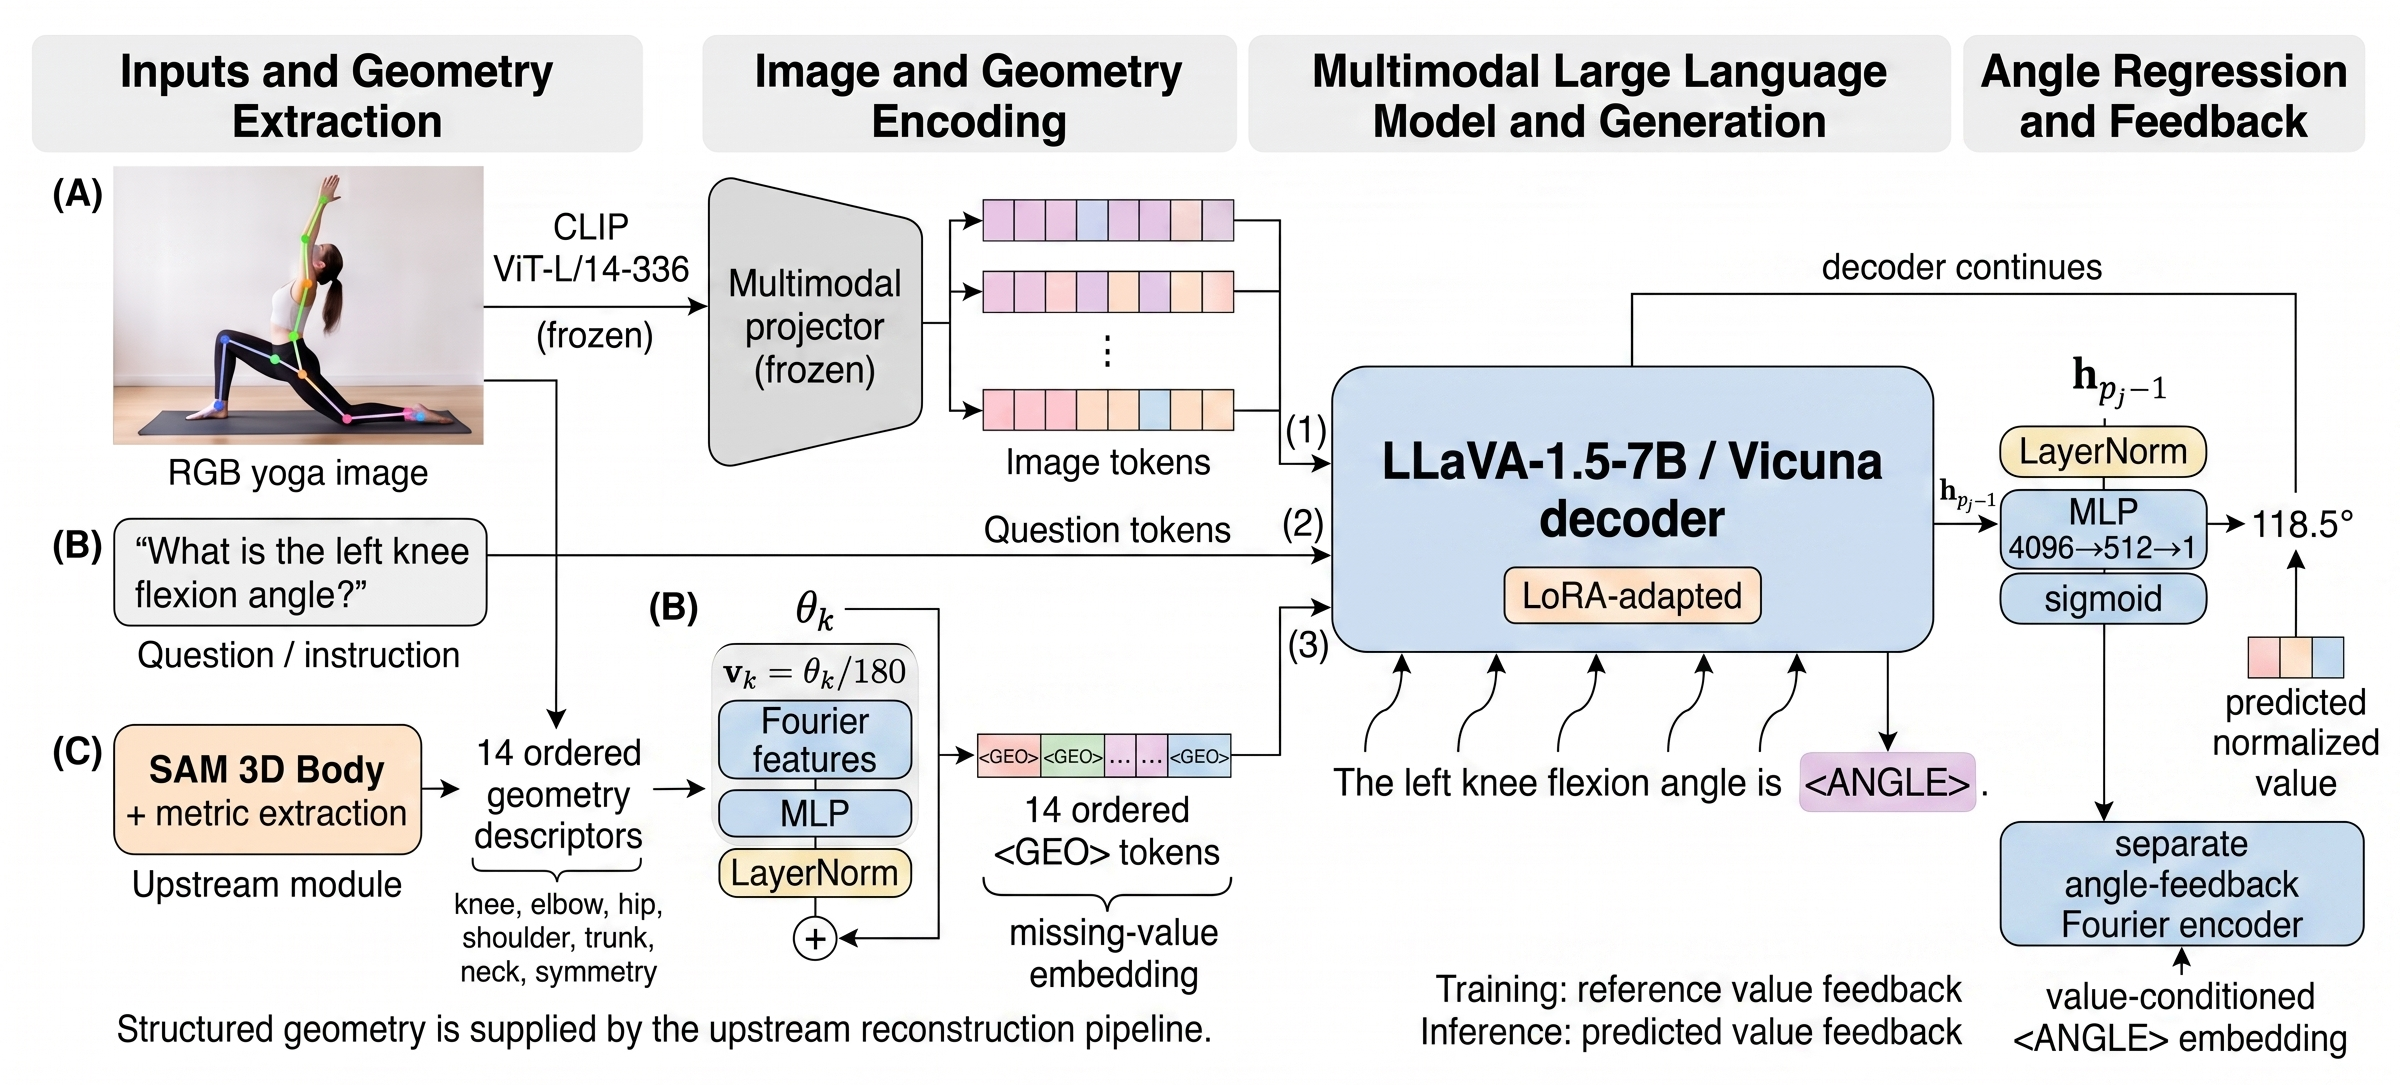
\includegraphics[width=0.98\textwidth]{method.png}
    \caption{Overview of YogaLLaVA V3. An input image is encoded by the frozen
    LLaVA vision encoder and projector, while an ordered set of degree-valued body descriptors
    is mapped to metric-aware \texttt{<GEO>} tokens. The causal language decoder
    attends jointly to visual, geometric, and textual context. When the decoder
    produces an \texttt{<ANGLE>} token, a regression head predicts the associated
    continuous value, which is embedded back into the sequence to condition
    subsequent generation.}
    \label{fig:yogallava_architecture}
\end{figure*}

\subsection{Structured Geometry Input}
\label{sec:structured_geometry_input}

YogaLLaVA V3 uses a fixed vocabulary of $K=14$ degree-valued descriptors.
The vocabulary covers left and right knee flexion, left and right elbow flexion, left and right hip opening, left and right shoulder elevation, trunk tilt, lateral trunk bend, trunk twist, neck alignment, knee symmetry, and elbow symmetry.
These descriptors form the angular subset of the broader geometric taxonomy introduced in Sec.~\ref{sec:dataset}.
Scale-dependent quantities, such as stance width and body-center offset, are not supplied to the model.
Hip symmetry is likewise not represented by a dedicated input descriptor, although three hip-symmetry targets occur in the held-out test set.

We represent the ordered geometry input as
\begin{equation}
    \mathcal{G}
    =
    \left\{(\theta_k,m_k)\right\}_{k=1}^{K},
    \qquad m_k\in\{0,1\},
    \label{eq:geometry_input}
\end{equation}
where $\theta_k$ is the $k$-th descriptor in degrees and $m_k$ indicates whether that measurement is available.
Explicitly modeling validity is necessary because a missing measurement is semantically distinct from a valid angle close to zero.

\subsection{Multimodal Geometry Representation}
\label{sec:geometry_representation}

\noindent\textbf{Visual and language inputs.}
The image is processed by the pretrained CLIP ViT-L/14-336 vision encoder in LLaVA.
Its patch-level features are projected into the language-model hidden space through the frozen multimodal projector.
The instruction and question are tokenized using the LLaVA tokenizer and combined with the projected visual features in the standard LLaVA input sequence.

To supply the geometry, we append exactly $K$ special \texttt{<GEO>} placeholders in a fixed canonical order.
Before decoding, the ordinary embeddings of these placeholders are replaced by geometry representations with the same dimensionality as the language-model hidden states.
Consequently, visual features, text tokens, and measurements are processed within a shared autoregressive sequence.

\noindent\textbf{Fourier encoding of continuous measurements.}
For every available descriptor, we normalize its value to $[0,1]$:
\begin{equation}
    v_k=\frac{\theta_k}{180}.
    \label{eq:angle_normalization}
\end{equation}
We encode $v_k$ with $B=16$ fixed, logarithmically spaced Fourier frequency bands instead of a single linear projection:
\begin{equation}
\begin{split}
    \boldsymbol{\phi}(v_k)=\big[
        &\sin(\omega_1v_k),\ldots,\sin(\omega_Bv_k),\\
        &\cos(\omega_1v_k),\ldots,\cos(\omega_Bv_k),v_k
    \big].
\end{split}
\label{eq:fourier_features}
\end{equation}
This mapping produces a $(2B+1)=33$ dimensional representation.
A two-layer MLP with hidden width 256 projects it to the $d=4096$ dimensional language-model space:
\begin{equation}
    \mathbf{z}_k
    =f_{\mathrm{geo}}\!\left(\boldsymbol{\phi}(v_k)\right),
    \qquad \mathbf{z}_k\in\mathbb{R}^{d}.
    \label{eq:scalar_projection}
\end{equation}

\noindent\textbf{Metric identity and missing values.}
The same scalar may carry different meanings for different anatomical measurements.
We therefore associate each descriptor with a learned metric-identity embedding $\mathbf{e}^{\mathrm{id}}_k\in\mathbb{R}^{d}$.
The final token for descriptor $k$ is
\begin{equation}
    \mathbf{g}_k=
    \begin{cases}
    \operatorname{LN}\!\left(
        \mathbf{e}^{\mathrm{id}}_k+\mathbf{z}_k
    \right), & m_k=1,\\[5pt]
    \operatorname{LN}\!\left(
        \mathbf{e}^{\mathrm{id}}_k+\mathbf{e}^{\mathrm{miss}}
    \right), & m_k=0,
    \end{cases}
    \label{eq:geometry_token}
\end{equation}
where $\mathbf{e}^{\mathrm{miss}}\in\mathbb{R}^{d}$ is a learned missing-value embedding and $\operatorname{LN}$ denotes layer normalization.
The ordered geometry sequence is
\begin{equation}
    \mathbf{G}=[\mathbf{g}_1,\ldots,\mathbf{g}_K]
    \in\mathbb{R}^{K\times d}.
    \label{eq:geometry_sequence}
\end{equation}
These vectors replace the corresponding \texttt{<GEO>} embeddings.
The decoder attends jointly to the image, question, and metric-specific continuous geometry.

\subsection{Angle-Aware Language Generation}
\label{sec:angle_generation}

Standard language models express numbers through discrete subword tokens.
Subword generation provides no explicit continuous prediction objective.
YogaLLaVA V3 instead introduces a special \texttt{<ANGLE>} token that separates numeric-slot placement from scalar-value estimation.
During training, every degree value in a geometry-grounded answer is replaced by \texttt{<ANGLE>}, and its normalized value is retained as a continuous target aligned with that token position.
For example,
\begin{quote}
\small
\textit{The left knee flexion angle is $140.2^\circ$.}
\end{quote}
is represented internally as
\begin{quote}
\small
\texttt{The left knee flexion angle is <ANGLE>.}
\end{quote}
The language decoder thus learns \emph{where} an angular value is required, whereas the regression branch learns \emph{which} value should occupy that position.

Let $p_j$ denote the position of the $j$-th \texttt{<ANGLE>} token.
Under causal decoding, the hidden state $\mathbf{h}_{p_j-1}$ produces the token at position $p_j$.
We predict its normalized value as
\begin{equation}
    \widehat{v}_j
    =\sigma\!\left(
        f_{\mathrm{reg}}(\mathbf{h}_{p_j-1})
    \right),
    \label{eq:angle_regression}
\end{equation}
where $f_{\mathrm{reg}}$ comprises layer normalization, a $4096\!\rightarrow\!512$ linear layer, GELU, and a $512\!\rightarrow\!1$ linear layer.
The sigmoid restricts predictions to $[0,1]$, after which the angle is recovered in degrees:
\begin{equation}
    \widehat{\theta}_j=180\widehat{v}_j.
    \label{eq:angle_denormalization}
\end{equation}
Using $\mathbf{h}_{p_j-1}$ ensures that the current value is estimated from the preceding causal context.
No value-conditioned embedding is placed at the current \texttt{<ANGLE>} position.

\noindent\textbf{Continuous-value feedback.}
After an angle slot is produced, its scalar value is re-embedded into the sequence so that subsequent language and later angle slots may condition on it.
An independent scalar encoder defines
\begin{equation}
    \mathbf{a}(u_j)
    =\mathbf{e}^{\mathrm{angle}}
    +f_{\mathrm{slot}}\!\left(\boldsymbol{\phi}(u_j)\right),
    \label{eq:angle_feedback}
\end{equation}
where $\mathbf{e}^{\mathrm{angle}}$ is a learned base embedding and $f_{\mathrm{slot}}$ is distinct from the geometry-input encoder $f_{\mathrm{geo}}$.
During teacher-forced training, $u_j$ is the reference normalized angle.
During autoregressive inference, $u_j=\widehat{v}_j$.
Accordingly, subsequent tokens condition on the reference value during training and on the model's own prediction at inference time.

\subsection{Joint Language and Geometry Learning}
\label{sec:training_objective}

We jointly optimize natural-language generation and continuous angle prediction.
Language supervision is restricted to the assistant response.
Image and geometry placeholders, the instruction, the question, and padding positions are excluded.
Let $\mathcal{T}$ denote the supervised assistant-token positions.
The causal language-modeling objective is
\begin{equation}
    \mathcal{L}_{\mathrm{LM}}
    =-\frac{1}{|\mathcal{T}|}
    \sum_{t\in\mathcal{T}}
    \log p_{\Theta}\!\left(
        y_t\mid y_{<t},I,q,\mathcal{G}
    \right).
    \label{eq:language_loss}
\end{equation}

For a minibatch containing $N$ supervised angle slots, the regression branch is optimized in normalized angle space using
\begin{equation}
    \mathcal{L}_{\mathrm{ang}}
    =\frac{1}{N}\sum_{j=1}^{N}
    \operatorname{SmoothL1}_{\beta}
    \!\left(\widehat{v}_j-v_j\right).
    \label{eq:regression_loss}
\end{equation}
The complete training objective is
\begin{equation}
    \mathcal{L}
    =\mathcal{L}_{\mathrm{LM}}
    +\lambda_{\mathrm{ang}}\mathcal{L}_{\mathrm{ang}},
    \label{eq:total_loss}
\end{equation}
with $\lambda_{\mathrm{ang}}=0.75$ and $\beta=0.05$, corresponding to a $9^\circ$ SmoothL1 transition in degree space.
The language term is causal cross-entropy with label smoothing.
Domain-knowledge records contain no \texttt{<ANGLE>} positions and therefore contribute only $\mathcal{L}_{\mathrm{LM}}$.

As a regularizer, we apply full geometry dropout to 15\% of geometry-grounded training records.
For a selected record, every measurement is marked unavailable and represented by the learned missing-value embedding.
We do not evaluate behavior under missing measurements at test time.

The CLIP vision encoder and multimodal projector remain frozen.
We adapt the Vicuna language decoder using LoRA with rank 32, scaling parameter 64, and dropout 0.10.
LoRA is applied to the $q$, $k$, $v$, and $o$ attention projections and to the gate, up, and down feed-forward projections.
The geometry encoder, angle-feedback encoder, learned angle embedding, regression head, and LoRA parameters are optimized jointly.
After adding \texttt{<GEO>} and \texttt{<ANGLE>} to the vocabulary, the input-embedding matrix and language-model output projection are also trainable.

\subsection{Autoregressive Inference}
\label{sec:inference}

At inference time, SAM 3D Body reconstruction provides the ordered geometry descriptors, while the frozen LLaVA vision encoder and projector process the input image.
The image, geometry tokens, instruction, and question are supplied without a reference answer.

Decoding proceeds autoregressively.
Ordinary tokens follow the standard LLaVA generation process.
When \texttt{<ANGLE>} is selected, the hidden state that produced it is passed to the regression head to obtain $\widehat{v}_j$.
The prediction is converted to degrees for the final response and encoded through Eq.~\eqref{eq:angle_feedback} as the embedding of that \texttt{<ANGLE>} token before decoding resumes.
After generation, the placeholders are replaced in order by their predicted degree values.
Token probabilities and scalar predictions are not averaged or combined at the output level.
The two interact through the slot-placement and continuous-value feedback mechanism.
\section{Experiments}
\label{sec:experimental_setup}

\subsection{Data Splits}
\label{sec:dataset_splits}

We train YogaLLaVA V3 on the combined domain-knowledge and geometry-grounded QA corpus introduced in Sec.~\ref{sec:dataset}.
The fixed splits contain 10,090 records and 10,177 supervised angle slots (Table~\ref{tab:dataset_splits}).
All evaluation below uses the geometry-grounded records.
The 200 held-out domain-knowledge records are reserved for future work, and we report no result on them.
The geometry-grounded subset is constructed from 3,000 images, with two QA records per image, and comprises 3,000 direct-angle, 905 comparison, 900 regional-summary, 600 misconception, and 595 instructor-observation examples.
Test images are excluded from training, while pose categories are shared across splits.
The resulting protocol evaluates generalization to unseen images of known asanas.
It does not test generalization to unseen pose categories.

\begin{table}[t]
    \centering
    \caption{Composition of the instruction-tuning corpus.}
    \label{tab:dataset_splits}
    \resizebox{\columnwidth}{!}{
    \begin{tabular}{lrrrr}
        \toprule
        \textbf{Split} &
        \textbf{Geometry QA} &
        \textbf{Domain QA} &
        \textbf{Total} &
        \textbf{Angle Slots} \\
        \midrule
        Train      & 5,396 & 3,690 & 9,086 & 9,163 \\
        Validation &   294 &   200 &   494 &   493 \\
        Test       &   310 &   200 &   510 &   521 \\
        \midrule
        Total      & 6,000 & 4,090 & 10,090 & 10,177 \\
        \bottomrule
    \end{tabular}}
\end{table}

\subsection{Implementation Details}
\label{sec:implementation_details}

YogaLLaVA V3 is initialized from LLaVA-1.5-7B.
Its CLIP ViT-L/14-336 image encoder operates at $336\!\times\!336$ resolution, and the multimodal projector maps the visual features to the 4,096-dimensional language space.
The maximum sequence length is 1,280 tokens.
Both the vision encoder and multimodal projector remain frozen.
The language decoder is adapted using the LoRA settings described in Sec.~\ref{sec:training_objective}, together with the geometry and angle components.

We train for 12 epochs using AdamW with weight decay 0.01 and gradient clipping at 1.0.
A per-device batch size of four and eight-step gradient accumulation produce an effective batch size of 32.
We use a cosine learning-rate schedule with linear warm-up over the first 3\% of optimizer updates.
The learning rates are $1.5\!\times\!10^{-4}$ for LoRA parameters, $2\!\times\!10^{-5}$ for the trainable input and output embeddings, and $1\!\times\!10^{-4}$ for the geometry encoder, angle-feedback encoder, angle embedding, and regression head.
The pretrained backbone is loaded in bfloat16, whereas the added numeric components are kept in float32.
Training is performed on one NVIDIA RTX A6000 GPU with fixed Python, NumPy, PyTorch, and CUDA seeds.

We evaluate the model after every epoch and select the checkpoint with the lowest teacher-forced validation angle RMSE.
The selected checkpoint obtains a validation RMSE of $19.83^\circ$, MAE of $12.63^\circ$, and $R^2$ of 0.874.
We report only the selected checkpoint.
Intermediate epoch-wise values serve as optimization diagnostics.

\subsection{Evaluation Protocol}
\label{sec:evaluation_protocol}

\noindent\textbf{Teacher-forced angle regression.}
Our primary numeric evaluation supplies the reference answer structure, including the number, positions, and ordering of \texttt{<ANGLE>} tokens, and evaluates the continuous prediction at each known slot.
Given $N$ reference angles $\theta_i$ and predictions $\widehat{\theta}_i$, we report MAE, RMSE, $R^2$, Pearson correlation, and the fractions of predictions within $5^\circ$, $10^\circ$, and $15^\circ$ of the references:
\begin{equation}
\operatorname{MAE}=\frac{1}{N}\sum_{i=1}^{N}
\left|\widehat{\theta}_i-\theta_i\right|,
\qquad
\operatorname{RMSE}=\sqrt{\frac{1}{N}\sum_{i=1}^{N}
(\widehat{\theta}_i-\theta_i)^2}.
\label{eq:evaluation_errors}
\end{equation}
Teacher forcing isolates continuous prediction given the correct linguistic slot structure.
It does not evaluate whether the model can produce, order, and correctly place the required slots on its own.

\noindent\textbf{Autoregressive generation.}
We also evaluate free-running generation on all 310 geometry-grounded test records.
YogaLLaVA V3 receives the image, question, and geometry input.
LLaVA-1.5-7B and Qwen2.5-VL-7B-Instruct~\cite{bai2025qwen25vl} are evaluated zero-shot using only the image and question.
The questions specify the target metrics and their expected order but do not reveal numeric values.
We report (i) slot-count accuracy over the full test set and (ii) numeric error on the common-success subset for which all models generate the correct number of values.
This distinction avoids comparing numeric errors computed on different model-specific subsets.

All numeric references are pseudo-measurements derived from SAM 3D Body.
They are not motion capture or manually verified biomechanical annotations.
Moreover, 518 of the 521 teacher-forced test targets are present in the structured geometry input.
The primary evaluation therefore measures question-conditioned descriptor selection, slot filling, reproduction, and linguistic expression.
It does not measure independent physical angle recovery from RGB images.
\section{Results}
\label{sec:results}

\subsection{Overall Angle-Slot Regression}
\label{sec:overall_results}

Teacher-forced regression covers 521 angle slots from 310 held-out geometry-grounded records.
YogaLLaVA V3 obtains an MAE of $13.98^\circ$ and an RMSE of $21.82^\circ$, with a Pearson correlation of 0.913.
The test $R^2$ is 0.832 and differs from the validation $R^2$ of 0.874 used for checkpoint selection (Sec.~\ref{sec:implementation_details}).
In addition, 57.01\% and 70.63\% of predictions fall within $10^\circ$ and $15^\circ$, respectively, of the reconstruction-derived references.
Table~\ref{tab:overall_results} in Appendix~\ref{app:additional_results} lists the full metric set.
These results indicate that the model can identify and express the requested measurement from the supplied geometry under a known answer structure.

Two reference points bound this result.
A constant predictor at the test mean attains an $R^2$ of 0 by construction.
The reported $R^2$ and RMSE imply a target standard deviation of $53.24^\circ$, which is that predictor's RMSE.
YogaLLaVA V3 reduces RMSE by 59\% against this anchor.
At the other end, 518 of the 521 targets are supplied among the geometry tokens (Sec.~\ref{sec:evaluation_protocol}).
An oracle that selects the correct descriptor and copies its value therefore attains an MAE of $0^\circ$ and an $R^2$ of 1 on those slots.
The distance from that upper bound measures how often the model selects the wrong descriptor or fails to reproduce a value it was given.


\subsection{Analysis by Question Type}
\label{sec:path_results}

Table~\ref{tab:path_results} reports performance across the five geometry-QA families.
Misconception questions achieve the lowest MAE ($11.28^\circ$) and highest within-$10^\circ$ accuracy (68.75\%), although this subset contains only 32 slots.
Regional-summary and comparison questions also perform favorably despite requiring multiple values or cross-body-part relations.
Instructor-observation questions are the most challenging, with an MAE of $21.08^\circ$ and within-$10^\circ$ accuracy of 25.81\%.
Their $R^2$ of 0.054 over 31 slots is the weakest result in the table and indicates that predictions in this family barely track their targets.
The error metrics alone understate this failure.
Their less explicit teacher-style formulations may make descriptor selection more ambiguous, although the present experiment does not isolate this factor.

\begin{table}[t]
    \centering
    \caption{Teacher-forced regression by geometry-QA type.}
    \label{tab:path_results}
    \resizebox{\columnwidth}{!}{
    \begin{tabular}{lrrrrr}
        \toprule
        \textbf{Question Type} & \textbf{Slots} &
        \textbf{RMSE $\downarrow$} & \textbf{MAE $\downarrow$} &
        \textbf{$R^2$ $\uparrow$} & \textbf{$\leq10^\circ$ $\uparrow$} \\
        \midrule
        Comparison & 106 & $21.53^\circ$ & $12.95^\circ$ & 0.791 & 62.26\% \\
        Direct angle & 155 & $22.65^\circ$ & $15.22^\circ$ & 0.821 & 51.61\% \\
        Instructor observation & 31 & $28.69^\circ$ & $21.08^\circ$ & 0.054 & 25.81\% \\
        Misconception & 32 & $17.10^\circ$ & $11.28^\circ$ & 0.877 & 68.75\% \\
        Region summary & 197 & $20.72^\circ$ & $12.88^\circ$ & 0.847 & 61.42\% \\
        \bottomrule
    \end{tabular}}
\end{table}

\subsection{Analysis by Geometric Descriptor}
\label{sec:metric_results}

Among descriptors with substantial test support, trunk twist yields the lowest MAE ($6.84^\circ$), followed by lateral trunk bend, trunk tilt, and right shoulder elevation (Table~\ref{tab:metric_results} in Appendix~\ref{app:additional_results}).
Left shoulder elevation is the most difficult descriptor, followed by elbow flexion and right hip opening.
These differences may arise from descriptor-specific distributions, reconstruction uncertainty, occlusion, or left--right ambiguity.
Identifying their individual effects requires further controlled analysis.

The symmetry categories contain only three or four slots and should not be used to draw broad conclusions.
Hip symmetry is also distinct because no dedicated hip-symmetry token is included in the 14-descriptor input vocabulary.
Its three test targets therefore cannot be retrieved from a corresponding independent input token.
Despite the missing token, hip symmetry reaches an MAE of $7.82^\circ$, lower than several descriptors with dedicated input tokens and far larger test support.
Under a retrieval-based reading of the regression, this direction is counterintuitive, and we note it as an open question given the three-slot sample.


\subsection{Autoregressive Generation}
\label{sec:generation_comparison}

Table~\ref{tab:generation_results} evaluates free-running generation.
YogaLLaVA V3 produces the correct number of numeric values for 267 of 310 records (86.1\%), compared with 66.1\% for LLaVA-1.5-7B and 68.1\% for Qwen2.5-VL-7B.
The Wilson 95\% confidence interval for YogaLLaVA V3 is $[81.8,89.5]\%$ and overlaps neither baseline interval ($[60.7,71.2]\%$ for LLaVA-1.5-7B and $[62.7,73.0]\%$ for Qwen2.5-VL-7B).
YogaLLaVA V3 is therefore more reliable at determining when and how many continuous outputs are required.

This comparison evaluates complete models.
It does not isolate a single architectural factor.
YogaLLaVA V3 receives the geometry input and task-specific instruction tuning, whereas the baselines are image-only and zero-shot.
The observed advantage reflects the combined effect of geometry conditioning, domain adaptation, and continuous angle regression.
It should not be read as a modality-matched ablation.

For numeric comparison, we use the 160-record common-success subset on which all three models produce the correct slot count.
Conditioning on joint success removes every record where a baseline produced an invalid slot count.
Because such records are plausibly the harder ones, the numeric gaps below hold conditional on this selection.
YogaLLaVA V3 achieves a slot-level MAE of $17.65^\circ$, compared with $42.80^\circ$ for LLaVA and $46.91^\circ$ for Qwen.
Its record-level macro MAE is $16.98^\circ$ with a 95\% bootstrap confidence interval of $[14.15,20.17]^\circ$.
The corresponding intervals are $[37.33,46.41]^\circ$ for LLaVA and $[41.59,53.87]^\circ$ for Qwen.
Paired bootstrap differences relative to YogaLLaVA are $24.85^\circ$ ($[19.45,30.35]^\circ$) for LLaVA and $30.64^\circ$ ($[23.70,37.83]^\circ$) for Qwen.

\begin{table}[t]
    \centering
    \caption{Autoregressive generation on 310 test records. Slot accuracy is
    measured on the full test set and reported with Wilson 95\% confidence
    intervals. Numeric errors use the 160-record common-success subset.}
    \label{tab:generation_results}
    \resizebox{\columnwidth}{!}{
    \begin{tabular}{lrrrr}
        \toprule
        \textbf{Model} & \textbf{Slot Match $\uparrow$} &
        \textbf{95\% CI} &
        \textbf{MAE $\downarrow$} & \textbf{RMSE $\downarrow$} \\
        \midrule
        YogaLLaVA V3 & 267/310 (86.1\%) & $[81.8,89.5]\%$ & $17.65^\circ$ & $27.23^\circ$ \\
        LLaVA-1.5-7B & 205/310 (66.1\%) & $[60.7,71.2]\%$ & $42.80^\circ$ & $52.59^\circ$ \\
        Qwen2.5-VL-7B & 211/310 (68.1\%) & $[62.7,73.0]\%$ & $46.91^\circ$ & $61.12^\circ$ \\
        \bottomrule
    \end{tabular}}
\end{table}

\subsection{Discussion and Limitations}
\label{sec:result_interpretation}

The teacher-forced and autoregressive evaluations characterize complementary capabilities.
The former measures continuous prediction at known answer slots, whereas the latter additionally requires the model to decide whether a numeric slot is needed, produce and order the correct number of slots, preserve consistency between numbers and language, and terminate appropriately.
Reporting them separately avoids conflating regression accuracy with generation quality.

The current evidence supports geometry-conditioned measurement selection and expression.
The references inherit uncertainty from monocular reconstruction, including viewpoint, occlusion, foreshortening, clothing, inversion, depth, and left--right ambiguities.
SAM 3D Body reports a mean per-joint position error of $54.8$~mm on 3DPW~\cite{yang2026sam3dbody}.
That figure is positional and does not convert to an angular tolerance.
No joint-angle error is published for the reconstruction, and we therefore cannot separate the share of the reported $13.98^\circ$ MAE that originates in the references themselves.
The references should not be interpreted as clinical, diagnostic, rehabilitation, motion-capture, or manually verified biomechanical ground truth.

The misconception and instructor-observation families place a further limitation on the present scope.
Both train the model to issue corrective, teacher-style judgments, and their supervision comes from the same measurements we decline to certify as clinically meaningful.
We have not checked the resulting corrections against expert instruction.
The generated judgments are therefore unvalidated as instructional advice.

The domain-knowledge set carries a separate caveat.
It supplies 4,090 of the 10,090 records and takes part in training, yet no experiment here measures whether the model answers questions about benefits, contraindications, or alignment cues correctly.
We therefore claim it as an annotation resource and make no accuracy claim for pose-level knowledge.

Finally, the experiments do not isolate modality contributions through ablation and do not test generalization to unseen yoga-pose categories.
These gaps, together with domain-knowledge evaluation, remain directions for future work.
\section{Conclusion}
\label{sec:conclusion}

We introduced YogaAlign, a geometry-grounded extension of Yoga-82, and YogaLLaVA V3, a vision--language model that integrates structured body measurements with continuous angle-aware generation.
YogaAlign combines pose-level domain knowledge with image-specific QA derived from reconstruction-based evidence paths.
YogaLLaVA V3 represents these measurements as metric-aware geometry tokens and predicts continuous values at angle slots.
The experiments demonstrate reliable question-conditioned selection and expression of supplied geometry under both teacher-forced and autoregressive evaluation.
They also define the present scope.
The evaluation covers the geometry-grounded set alone.
YogaLLaVA V3 reasons over monocular reconstruction-derived measurements and is not a substitute for independently validated biomechanical assessment.
Future work should evaluate the domain-knowledge set, modality-matched ablations, human-verified geometric references, pose-held-out generalization, and the consistency of generated corrections with expert instruction.
\appendices

\section{Annotation Sets and Evidence Representations}
\label{app:annotation_sets}

Table~\ref{tab:qa_annotation_overview} contrasts the evidence sources and supervision targets of the two QA sets.

\begin{table*}[t]
\centering
\caption{Complementary QA annotation sets in YogaAlign.}
\label{tab:qa_annotation_overview}
\small
\setlength{\tabcolsep}{4pt}
\renewcommand{\arraystretch}{1.15}
\begin{tabularx}{\textwidth}{L{0.19\textwidth} L{0.26\textwidth} L{0.30\textwidth} X}
\toprule
\textbf{QA set} & \textbf{Primary evidence} & \textbf{Question scope} & \textbf{Supervision target} \\
\midrule
Domain knowledge &
Pose-specific text collected from online yoga sources &
Identity, benefits, contraindications, precautions, procedures, alignment cues,
modifications, breathing, mistakes, corrections, and sequencing &
Pose-level semantic and instructional reasoning. \\
Geometry grounded &
Degree-valued measurements extracted for an individual image &
Joint flexion, hip opening, shoulder elevation, trunk configuration, angular
symmetry, regional summaries, and measured-condition verification &
Image-specific measurement selection, comparison, interpretation, and numeric expression. \\
\bottomrule
\end{tabularx}
\end{table*}


\section{Domain-Knowledge Generation Procedure}
\label{app:domain_generation}

We use Crawl4AI to retrieve and extract text from pose-relevant online sources for each of the 82 categories.
We retain information relevant to pose understanding and instruction, including execution steps, alignment principles, modifications, breathing cues, common mistakes, corrections, benefits, contraindications, and precautions.
We exclude navigation text, advertisements, author biographies, publication metadata, product promotions, and generic marketing language.
Each pose document is then divided into 5,000-character chunks with a 500-character overlap.

The extractor produces two representations per chunk (Table~\ref{tab:domain_knowledge_representation}).
Relational facts encode single subject--relation--object statements suited to concise factual questions.
Knowledge units retain multi-step or explanatory content suited to procedural, alignment, safety, modification, breathing, sequencing, and correction questions.

We instruct the generator to use only the supplied evidence.
Compact signatures of previously extracted facts, knowledge units, and questions are maintained across chunks to suppress semantic repetition.
Question families are varied across factual, procedural, scenario-based, safety, reverse-lookup, correction, and teacher-cue formulations.
Each accepted item stores the pose, source-chunk identifier, question, answer, QA type, supporting facts, supporting knowledge units, and an evidence phrase.

\begin{table*}[t]
\centering
\caption{Intermediate evidence representations for domain-knowledge QA generation.}
\label{tab:domain_knowledge_representation}
\small
\setlength{\tabcolsep}{4pt}
\renewcommand{\arraystretch}{1.15}
\begin{tabularx}{\textwidth}{L{0.21\textwidth} L{0.27\textwidth} L{0.28\textwidth} X}
\toprule
\textbf{Representation} & \textbf{Role} & \textbf{Typical content} & \textbf{Supported QA form} \\
\midrule
Relational facts &
Single-fact, evidence-backed statements &
Names, difficulty, benefits, contraindications, precautions, props, muscles,
modifications, and related poses &
Concise factual and reverse-lookup questions. \\
Structured knowledge units &
Multi-sentence or multi-step evidence &
Procedures, alignment, safety, modifications, mistakes, corrections, breathing,
sequencing, and teaching cues &
Explanatory, procedural, scenario-based, and teacher-style questions. \\
\bottomrule
\end{tabularx}
\end{table*}

\section{Annotation Generation Settings}
\label{app:generation_settings}

Tables~\ref{tab:domain_qa_config} and~\ref{tab:geometry_qa_settings} record the values used to generate the two QA sets described in Sec.~\ref{subsec:qa_generation}.
We fixed every value before generation and did not tune any of them against a held-out measurement.
The tables are reported for reproduction and carry no claim of optimality.

\begin{table}[h]
\centering
\caption{Domain-knowledge QA generation settings.}
\label{tab:domain_qa_config}
\small
\setlength{\tabcolsep}{4pt}
\renewcommand{\arraystretch}{1.10}
\begin{tabular}{ll}
\toprule
\textbf{Item} & \textbf{Setting} \\
\midrule
Knowledge organization & One document per pose \\
Chunk size / overlap & 5,000 / 500 characters \\
Maximum relational facts per chunk & 8 \\
Maximum knowledge units per chunk & 3 \\
Maximum QA pairs per chunk & 10 \\
Maximum QA pairs per knowledge unit & 3 \\
Generation temperature & 0 \\
Context length & 32,768 tokens \\
\bottomrule
\end{tabular}
\end{table}

\begin{table}[h]
\centering
\caption{Geometry-grounded QA generation settings.}
\label{tab:geometry_qa_settings}
\small
\setlength{\tabcolsep}{4pt}
\renewcommand{\arraystretch}{1.10}
\begin{tabular}{ll}
\toprule
\textbf{Item} & \textbf{Setting} \\
\midrule
Input representation & Per-image metric record \\
Evidence representation & Metric facts and graph paths \\
Selected images & 3,000 \\
Image selection & Balanced-proportional sampling \\
QA pairs per image & 2 \\
LLM & Qwen3.6-35B-A3B~\cite{qwen2026qwen36} \\
Context length & 16,000 tokens \\
Temperature & 0.15 \\
Maximum regeneration attempts & 2 \\
Primary supervision & Exact angles in degrees \\
Diversity control & Rolling memory and family rotation \\
Quality control & Rule validation and deterministic templates \\
\bottomrule
\end{tabular}
\end{table}

\section{Additional Regression Results}
\label{app:additional_results}

Table~\ref{tab:overall_results} lists the full metric set for the teacher-forced evaluation of Sec.~\ref{sec:overall_results}.
Table~\ref{tab:metric_results} breaks the same slots down by target descriptor.
Ten of the fifteen descriptors carry more than thirty slots, and the three symmetry rows carry three or four.

\begin{table}[h]
    \centering
    \caption{Teacher-forced angle-slot regression on the held-out test set.
    Errors are measured against SAM 3D Body-derived pseudo-measurements.}
    \label{tab:overall_results}
    \begin{tabular}{lr}
        \toprule
        \textbf{Metric} & \textbf{YogaLLaVA V3} \\
        \midrule
        Angle slots & 521 \\
        RMSE $\downarrow$ & $21.82^\circ$ \\
        MAE $\downarrow$ & $13.98^\circ$ \\
        $R^2$ $\uparrow$ & 0.832 \\
        Pearson $r$ $\uparrow$ & 0.913 \\
        Within $5^\circ$ $\uparrow$ & 34.36\% \\
        Within $10^\circ$ $\uparrow$ & 57.01\% \\
        Within $15^\circ$ $\uparrow$ & 70.63\% \\
        \bottomrule
    \end{tabular}
\end{table}

\begin{table}[h]
    \centering
    \caption{Teacher-forced regression by target descriptor.}
    \label{tab:metric_results}
    \resizebox{\columnwidth}{!}{
    \begin{tabular}{lrrr}
        \toprule
        \textbf{Descriptor} & \textbf{Slots} &
        \textbf{RMSE $\downarrow$} & \textbf{MAE $\downarrow$} \\
        \midrule
        Knee symmetry & 4 & $3.23^\circ$ & $2.68^\circ$ \\
        Elbow symmetry & 4 & $6.90^\circ$ & $5.53^\circ$ \\
        Hip symmetry & 3 & $10.18^\circ$ & $7.82^\circ$ \\
        Trunk twist & 33 & $11.02^\circ$ & $6.84^\circ$ \\
        Lateral trunk bend & 38 & $14.92^\circ$ & $9.24^\circ$ \\
        Right shoulder elevation & 34 & $14.82^\circ$ & $9.89^\circ$ \\
        Trunk tilt & 34 & $15.48^\circ$ & $9.50^\circ$ \\
        Neck alignment & 37 & $17.34^\circ$ & $12.75^\circ$ \\
        Left hip opening & 48 & $18.40^\circ$ & $13.28^\circ$ \\
        Right knee flexion & 51 & $22.55^\circ$ & $12.09^\circ$ \\
        Left knee flexion & 47 & $23.66^\circ$ & $15.56^\circ$ \\
        Right elbow flexion & 50 & $24.80^\circ$ & $18.39^\circ$ \\
        Right hip opening & 48 & $25.41^\circ$ & $17.36^\circ$ \\
        Left elbow flexion & 47 & $27.77^\circ$ & $18.46^\circ$ \\
        Left shoulder elevation & 43 & $31.22^\circ$ & $21.23^\circ$ \\
        \bottomrule
    \end{tabular}}
\end{table}
\clearpage

\bibliographystyle{IEEEtran}
\bibliography{references}

\end{document}
